\documentclass[11pt,a4paper]{report}
\usepackage[utf8]{inputenc}
\usepackage{amsmath}
\usepackage{graphicx}
\usepackage{gensymb}
\usepackage{listings}
\usepackage{tikz}
\usepackage{pgfplots}
\usepackage{mathtools}
\usetikzlibrary{arrows,positioning}
\tikzset{
    %Define standard arrow tip
    >=stealth',
    % Define arrow style
    pil/.style={
           ->,
           thick,
           shorten <=2pt,
           shorten >=2pt,}
}
\usepackage{geometry}
\geometry{
    left=2cm,
    right=0.64cm,
    top=0.64cm,
    bottom=2cm
}
\usepackage{multicol}
\setlength{\columnsep}{1cm}
\graphicspath{ {images/} }

\begin{document}

\chapter{Semester 2 Examination 2012-2013\\CZ4034 Information Retrieval}
\begin{multicols*}{2}

\section{Question 1}

\noindent \textbf{Question 1a} Write down the expanded biagram and permuterm queries for the following queries by filling in line 3 onwards in table below. Follow the example shown in the second row of the table.

\begin{center}
\begin{tabular}{| l | l | l | l |}
    \hline
    Part      & Wilcard Query & Bigrams    & Permuterms \\
    \hline
    e.g       & SH*           & \$S, SH     & \$SH* \\
    (i)       & N*T*U         & \$N, T, U\$ & U\$N* \\
    (ii)      & S*T           & \$S, T\$    & T\$S* \\
    (iii)     & *H*T          & H, T\$      & T\$*  \\
    (iv)      & *H*           & H           & H*    \\
    (v)       & S*I*T         & \$S, I, T   & \$S*  \\
    \hline
\end{tabular}
\end{center}

\noindent For (i) (iii) and (v), after searching for terms using the permuterms, we do exhausted filter on each terms.\\

\noindent \textbf{Question 1b} Using your answers in Q1(a) as examples where applicable: \\

\noindent \textbf{(i)} Name two advantages of permuterm over bigram

\noindent Advantage 1: Permuterm is more efficient than bigram, for example, in Q1a(i) we need to do 2 search in two binary tree when using bigram approach, but we only need to do 1 search in 1 permuterm index when using permuterm approach.

\noindent Advantage 2: [Need help!]\\

\noindent \textbf{(ii)} Name one advantage of bigrams over permuterms

\noindent Answer: The index size bigram is smaller than permuterm.\\

\noindent \textbf{(iii)} Describe the post-processing operations needed to weed out false matches for both bigram and permuterm approaches.

\noindent Answer: For bigram, we need to find intersection of terms in all result lists by using merging algorithm. For permuterms, we need to do exhausted filters for query with more than one *.\\

\noindent \textbf{Question 1c} Suppose you are given two postings list for term X and term Y. Consider the following Boolean query.

\begin{center}
\verb|(NOT X) AND (NOT Y)|
\end{center}

\noindent \textbf{(i)} Write a postings merge algorithm in pseudocode or describe in English the steps of your algorithm.

\noindent Answer: since the boolean expression is equivalent to \verb|NOT( X OR Y )|, the algorithm:

\begin{lstlisting}
define ALL_DATA
XY = Merge X and Y without duplication
Remove elements of XY from ALL_DATA
\end{lstlisting}

\noindent Note: the real answer should be longer than this, specifically, the last steps need to elaboration. \\

\noindent \textbf{(ii)} If $x$ and $y$ are the lengths of posting X and Y, respectively, what is the complexity of your merge algorithm in Big O notation? Hint: normal merge complexity is $O(x+y)$.

\noindent Answer: We need $O(x+y)$ complexity to merge X and Y. To remove $x+y$ data from a list with $n$ elements, we need $O((x+y)+n)$. Hence, the worse case complexity for the algorithm is $O(x+y+n)$.

\section{Question 2}

\noindent \textbf{Question 2a} In Single-Pass In-Memory Indexing (SPIMI), each block maintains its own dictionary of terms. When memory is exhausted, the block is written to the disk\\

\noindent \textbf{(i)} Explain why each block's term dictionary must be sorted prior to writing block to the disk.

\noindent Not in syllabus\\

\noindent \textbf{(ii)} Is each postings list sorted in ascending doc ID order? Justify your answer.

\noindent Not in syllabus\\

\noindent \textbf{Question 2b} The top 10 retrieval results for two search engines SE1 and SE2 are shown below (1=relevant, 0=irrelevant) where the leftmost item is the top ranked search result. Assume there are 4 relevant documents.

\begin{center}
\begin{tabular}{ l l l l l l l l l l l l}
    SE1 & 1 & 0 & 1 & 0 & 0 &  & 0 & 0 & 0 & 1 & 1 \\
    SE2 & 0 & 1 & 0 & 0 & 1 &  & 1 & 1 & 0 & 0 & 0 \\
\end{tabular}
\end{center}

\noindent \textbf{(i)} Compute the Mean Average Precision of each search engine.

\noindent Answer: For SE1

$$\text{Precision@1}=1$$
$$\text{Precision@3}=2/3$$
$$\text{Precision@9}=3/9$$
$$\text{Precision@10}=4/10$$
$$\text{MAP} = \frac{1}{4} \cdot (1 + \frac{2}{3} + \frac{3}{9} + \frac{4}{10})= 0.60$$

\noindent For SE2:

$$\text{Precision@2}=1/2$$
$$\text{Precision@5}=2/5$$
$$\text{Precision@6}=3/6$$
$$\text{Precision@7}=4/7$$
$$\text{MAP} = \frac{1}{4} \cdot (\frac{1}{2} + \frac{2}{5} + \frac{3}{6} + \frac{4}{7}) = 0.49$$

\noindent \textbf{(ii)} Compute the R-precision of each search engine.

\noindent Answer: For a given query topic $Q$, R-precision is the precision at $R$, where $R$ is the number of relevant documents for $Q$. In other words, if there are $r$ relevant documents among the top-R retrieved documents, then R-precision is $r/R$.\\

\noindent For this question, the R-precision for SE1 and SE2 are:

$$\text{SE1, Precision@4}=2/4$$
$$\text{SE2, Precision@4}=1/4$$

\noindent \textbf{(iii)} Which search engine is better? Explain your answer.

\noindent Answer: according to MAP of two search engine, SE1 is better because it has higher MAP. \\

\noindent \textbf{Question 2c} Consider the following XML fragment:

\begin{lstlisting}[language=XML]
<person>
    <firstname>John Middle</firstname>
    <lastname>Doe</lastname>
    <email>john.doe@gmail.com</email>
</person>
\end{lstlisting}

\noindent \textbf{(i)} Enumerate \underline{all} structural terms for this XML fragment by fillling in table below. Apply case-folding and punctuation-removal, using a word as the base unit. The first three structural terms have been enumerated for you

\begin{center}
\begin{tabular}{| l | l | l |}
    \hline
    Term & Lexicalized & Lexicalize \\
         & sutree 1    & subtree 2  \\
    \hline
    \verb|"john"| & \verb|/firstname#| & \verb|/person/|\\
                  & \verb|"john"|      & \verb|firstname#"john"| \\
    \hline
\end{tabular}
\end{center}

\noindent Not in syllabus\\

\noindent \textbf{(ii)} How many dimensions are needed if the vector space model is used to represent this XML fragment via the structural terms? That is, how many terms are there in the vocabulary/lexicon?

\noindent Not in syllabus\\

\noindent \textbf{(iii)} Using each XML fragment as a ``document'', and assuming that the \verb|<email>| fragment has a lower weight/importance than \verb|<lastname>|, list the returned full lexicalized subtrees in descending order of similarity for the query ``doe''.

\noindent Not in syllabus

\section{Question 3}

\noindent \textbf{Question 3a} Consider the seven restaurant reviews in table below, where the reviews are classified into two classes (i.e. positive, negative).

\begin{center}
\begin{tabular}{| l | p{5cm} | l |}
    \hline
    ID  & Review & Sentiment \\ \hline
    1   & nice food nice service & Positive \\
    2   & food is good as expected & Positive \\
    3   & can not wait to go back & Positive \\
    4   & must try & Positive \\
    5   & food is nice but not as good as expected & Negative \\
    6   & do not want to go back & Negative \\
    7   & do not want to wait long & Negative \\
    \hline
\end{tabular}
\end{center}

\noindent \textbf{(i)} Build a multinomial Naive Bayes classifier with the reviews in the table. You may use words as features.

\noindent Answer: The number of vocabulary is 19, i.e. \verb|as|, \verb|back|, \verb|but|, \verb|can|, \verb|do|, \verb|expected|, \verb|food|, \verb|go|, \verb|good|, \verb|is|, \verb|long|, \verb|must|, \verb|nice|, \verb|not|, \verb|service|, \verb|to|, \verb|try|, \verb|wait|, \verb|want|.

$$ P(\text{as} | \text{Postive} ) = \frac{1+ 1}{17 + 19} = \frac{2}{36}$$
$$ P(\text{back} | \text{Postive} ) = \frac{1+ 1}{17 + 19} = \frac{2}{36}$$
$$ P(\text{but} | \text{Postive} ) = \frac{0+ 1}{17 + 19} = \frac{1}{36}$$
$$ P(\text{can} | \text{Postive} ) = \frac{1+ 1}{17 + 19} = \frac{2}{36}$$
$$ P(\text{do} | \text{Postive} ) = \frac{0+ 1}{17 + 19} = \frac{1}{36}$$
$$ P(\text{expected} | \text{Postive} ) = \frac{1+ 1}{17 + 19} = \frac{2}{36}$$
$$ P(\text{food} | \text{Postive} ) = \frac{2+ 1}{17 + 19} = \frac{3}{36}$$
$$ P(\text{go} | \text{Postive} ) = \frac{1+ 1}{17 + 19} = \frac{2}{36}$$
$$ P(\text{good} | \text{Postive} ) = \frac{1+ 1}{17 + 19} = \frac{2}{36}$$
$$ P(\text{is} | \text{Postive} ) = \frac{1+ 1}{17 + 19} = \frac{2}{36}$$
$$ P(\text{long} | \text{Postive} ) = \frac{0+ 1}{17 + 19} = \frac{1}{36}$$
$$ P(\text{must} | \text{Postive} ) = \frac{1+ 1}{17 + 19} = \frac{2}{36}$$
$$ P(\text{nice} | \text{Postive} ) = \frac{2+ 1}{17 + 19} = \frac{3}{36}$$
$$ P(\text{not} | \text{Postive} ) = \frac{1+ 1}{17 + 19} = \frac{2}{36}$$
$$ P(\text{service} | \text{Postive} ) = \frac{1+ 1}{17 + 19} = \frac{2}{36}$$
$$ P(\text{to} | \text{Postive} ) = \frac{1+ 1}{17 + 19} = \frac{2}{36}$$
$$ P(\text{try} | \text{Postive} ) = \frac{1+ 1}{17 + 19} = \frac{2}{36}$$
$$ P(\text{wait} | \text{Postive} ) = \frac{1+ 1}{17 + 19} = \frac{2}{36}$$
$$ P(\text{want} | \text{Postive} ) = \frac{0+ 1}{17 + 19} = \frac{1}{36}$$

$$ P(\text{as} | \text{Negative} ) = \frac{2 + 1}{21 + 19} = \frac{3}{40}$$
$$ P(\text{back} | \text{Negative} ) = \frac{1 + 1}{21 + 19} = \frac{2}{40}$$
$$ P(\text{but} | \text{Negative} ) = \frac{1 + 1}{21 + 19} = \frac{2}{40}$$
$$ P(\text{can} | \text{Negative} ) = \frac{0 + 1}{21 + 19} = \frac{1}{40}$$
$$ P(\text{do} | \text{Negative} ) = \frac{2 + 1}{21 + 19} = \frac{3}{40}$$
$$ P(\text{expected} | \text{Negative} ) = \frac{1 + 1}{21 + 19} = \frac{2}{40}$$
$$ P(\text{food} | \text{Negative} ) = \frac{1 + 1}{21 + 19} = \frac{2}{40}$$
$$ P(\text{go} | \text{Negative} ) = \frac{1 + 1}{21 + 19} = \frac{2}{40}$$
$$ P(\text{good} | \text{Negative} ) = \frac{1 + 1}{21 + 19} = \frac{2}{40}$$
$$ P(\text{is} | \text{Negative} ) = \frac{1 + 1}{21 + 19} = \frac{2}{40}$$
$$ P(\text{long} | \text{Negative} ) = \frac{1 + 1}{21 + 19} = \frac{2}{40}$$
$$ P(\text{must} | \text{Negative} ) = \frac{0 + 1}{21 + 19} = \frac{1}{40}$$
$$ P(\text{nice} | \text{Negative} ) = \frac{1 + 1}{21 + 19} = \frac{2}{40}$$
$$ P(\text{not} | \text{Negative} ) = \frac{3 + 1}{21 + 19} = \frac{4}{40}$$
$$ P(\text{service} | \text{Negative} ) = \frac{0 + 1}{21 + 19} = \frac{1}{40}$$
$$ P(\text{to} | \text{Negative} ) = \frac{2 + 1}{21 + 19} = \frac{3}{40}$$
$$ P(\text{try} | \text{Negative} ) = \frac{0 + 1}{21 + 19} = \frac{1}{40}$$
$$ P(\text{wait} | \text{Negative} ) = \frac{1 + 1}{21 + 19} = \frac{2}{40}$$
$$ P(\text{want} | \text{Negative} ) = \frac{2 + 1}{21 + 19} = \frac{3}{40}$$

\noindent \textbf{(ii)} Classify the following review by using the Naive Bayes classifier of Q3(a)(i):
\begin{center}\verb|want to go back back|\end{center}

\scriptsize
$$P(\text{Positive}|d) = \frac{1}{P(d)} \frac{1}{36} \cdot \frac{2}{36} \cdot \frac{2}{36} \cdot (\frac{2}{36})^2 \cdot \frac{4}{7}= 0.151 \times 10^{-6}$$

$$P(\text{Negative}|d) = \frac{1}{P(d)} \frac{3}{40} \cdot \frac{3}{40} \cdot \frac{2}{40} \cdot (\frac{2}{40})^2  \cdot \frac{3}{7}= 0.301 \times 10^{-6}$$
\normalsize

\noindent Since $P(\text{Negative}|d) > P(\text{Positive}|d)$, we classify the review as Negative.\\

\noindent \textbf{(iii)} Classify the following review with the Rocchio classification method using the reviews in the table as training data
\begin{center}\verb|food is not nice food|\end{center}

\noindent Answer: Before normalize
\scriptsize
\begin{center}
\begin{tabular}{| l | l l l l l l l |}
\hline
Term     & ID1 & ID2 & ID3 & ID4 & ID5 & ID6 & ID7 \\ \hline
as       & 0   & 1   & 0   & 0   & 2   & 0   & 0   \\
back     & 0   & 0   & 1   & 0   & 0   & 1   & 0   \\
but      & 0   & 0   & 0   & 0   & 1   & 0   & 0   \\
can      & 0   & 0   & 1   & 0   & 0   & 0   & 0   \\
do       & 0   & 0   & 0   & 0   & 0   & 1   & 1   \\
expected & 0   & 1   & 0   & 0   & 1   & 0   & 0   \\
food     & 1   & 1   & 0   & 0   & 1   & 0   & 0   \\
go       & 0   & 0   & 1   & 0   & 0   & 1   & 0   \\
good     & 0   & 1   & 0   & 0   & 1   & 0   & 0   \\
is       & 0   & 1   & 0   & 0   & 1   & 0   & 0   \\
long     & 0   & 0   & 0   & 0   & 0   & 0   & 1   \\
must     & 0   & 0   & 0   & 1   & 0   & 0   & 0   \\
nice     & 2   & 0   & 0   & 0   & 1   & 0   & 0   \\
not      & 0   & 0   & 1   & 0   & 1   & 1   & 1   \\
service  & 1   & 0   & 0   & 0   & 0   & 0   & 0   \\
to       & 0   & 0   & 1   & 0   & 0   & 1   & 1   \\
try      & 0   & 0   & 0   & 1   & 0   & 0   & 0   \\
wait     & 0   & 0   & 1   & 0   & 0   & 0   & 1   \\
want     & 0   & 0   & 0   & 0   & 0   & 1   & 1   \\ \hline
\end{tabular}
\end{center}
\normalsize

\clearpage
\noindent We do a normalization without TF-IDF (you can do TF-IDF too).

\scriptsize
\begin{center}
\begin{tabular}{| l | l l l l l l l |}
\hline
Term     & ID1  & ID2  & ID3  & ID4  & ID5  & ID6  & ID7 \\ \hline
as       & 0    & 0.45 & 0    & 0    & 0.60 & 0    & 0   \\
back     & 0    & 0    & 0.41 & 0    & 0    & 0.41 & 0   \\
but      & 0    & 0    & 0    & 0    & 0.30 & 0    & 0   \\
can      & 0    & 0    & 0.41 & 0    & 0    & 0    & 0   \\
do       & 0    & 0    & 0    & 0    & 0    & 0.41 & 0.41\\
expected & 0    & 0.45 & 0    & 0    & 0.30 & 0    & 0   \\
food     & 0.41 & 0.45 & 0    & 0    & 0.30 & 0    & 0   \\
go       & 0    & 0    & 0.41 & 0    & 0    & 0.41 & 0   \\
good     & 0    & 0.45 & 0    & 0    & 0.30 & 0    & 0   \\
is       & 0    & 0.45 & 0    & 0    & 0.30 & 0    & 0   \\
long     & 0    & 0    & 0    & 0    & 0    & 0    & 0.41\\
must     & 0    & 0    & 0    & 0.71 & 0    & 0    & 0   \\
nice     & 0.82 & 0    & 0    & 0    & 0.30 & 0    & 0   \\
not      & 0    & 0    & 0.41 & 0    & 0.30 & 0.41 & 0.41\\
service  & 0.41 & 0    & 0    & 0    & 0    & 0    & 0   \\
to       & 0    & 0    & 0.41 & 0    & 0    & 0.41 & 0.41\\
try      & 0    & 0    & 0    & 0.71 & 0    & 0    & 0   \\
wait     & 0    & 0    & 0.41 & 0    & 0    & 0    & 0.41\\
want     & 0    & 0    & 0    & 0    & 0    & 0.41 & 0.41\\ \hline
\end{tabular}
\end{center}
\normalsize

\noindent I do not finish the solution for this answer, it takes too long to finish. \\

\noindent \textbf{Question 3b} Calculate the macro-averaged and micro-average F-measure of the text classification system whose results on two classes are shown in the following tables:

\noindent For class A:
\begin{center}
\begin{tabular}{| l | l | l |}
\hline
             & Truth: Yes & Truth No \\ \hline
System: Yes  & 4  & 8 \\ \hline
System: No   & 10 & 28\\ \hline
\end{tabular}
\end{center}

\noindent For class B:
\begin{center}
\begin{tabular}{| l | l | l |}
\hline
             & Truth: Yes & Truth No \\ \hline
System: Yes  & 12 & 4  \\ \hline
System: No   & 8  & 26 \\ \hline
\end{tabular}
\end{center}

$$P_A = \frac{4}{12}$$
$$R_A = \frac{4}{14}$$
$$F_A = \frac{2PR}{P+R} = \frac{4}{13}$$

$$P_B = \frac{12}{16}$$
$$R_B = \frac{12}{20}$$
$$F_B = \frac{2PR}{P+R} = \frac{2}{3}$$

\noindent For macro-averaging, the weight is the same:

$$F = \frac{1}{2} \cdot \frac{4}{13} + \frac{1}{2} \cdot \frac{2}{3} = 0.487$$

\noindent For micro-averaging:

$$P = \frac{4 + 12}{12 + 16} = \frac{16}{28}$$
$$R = \frac{4 + 12}{14 + 20} = \frac{16}{34}$$
$$F = 0.516$$

\noindent \textbf{Question 3c} If we have very little data for training a text classification system, what approaches can we use to solve the problem?

\noindent Answer: Fist, we can solve the problem by collecting more data. Second, since overfitting problem will occur when training data are small, we can use cross-validation technique and regularization technique to avoid overfitting. Third, we can do random subsampling or bootstrapping. \\

\noindent \textbf{Question 4a} Cluster the following six vectors into two cluster by using the K-Means algorithm, supposing that the initial seeds are A1 and A6:

$$A1=(1,4), A2=(2,6)$$
$$A3=(5,8), A4=(5,3)$$
$$A5=(6,6), A6=(7,4)$$

\begin{tikzpicture}
\begin{axis}[
    enlargelimits=false,
    axis equal
]
\addplot+[
    nodes near coords,
    only marks,
    point meta=explicit symbolic
]
table[meta=label] {
    x y label
    1 4 A1
    2 6 A2
    5 8 A3
    5 3 A4
    6 6 A5
    7 4 A6
};
\end{axis}
\end{tikzpicture}

\noindent After the first iteration, $A1$ and $A2$ in one cluster, and the rest in another cluster.

$$\mu_1 = [1.5,5]$$
$$\mu_2 = [5.75, 5.25]$$

\begin{tikzpicture}
\begin{axis}[
    enlargelimits=false,
    axis equal
]
\addplot+[
    nodes near coords,
    only marks,
    point meta=explicit symbolic
]
table[meta=label] {
    x y label
    1 4 A1
    2 6 A2
    5 8 A3
    5 3 A4
    6 6 A5
    7 4 A6
    1.5 5 $\mu_1$
    5.75 5.25 $\mu_2$
};
\end{axis}
\end{tikzpicture}

\noindent The algorithm converges after first iteration. \\

\noindent \textbf{Question 4b} Describe the algorithm of Hierarchical Agglomerative Clustering. Illustrate TWO ways of measuring cluster similarity with examples

\noindent Answer: Hierarchical Agglomerative Clustering is a bottom-up approach. It starts with $N$ clusters, where $N$ is the total number of data. Then, it repeatively merging two closest clusters and update the proximity matrix. The first way to measure cluster similarity is Euclidean distance:
$$\text{dist}(d1,d2)=\sqrt{\sum_{i=1}^D (d1_{i} - d2_{i})^2}$$

\noindent The second way to measure cluster similarity is Cosine Similarity:
$$\text{cosine}(\vec{d1},\vec{d2}) = \frac{\vec{d1} \cdot \vec{d2}}{|\vec{d1}||\vec{d2}|}$$

\noindent For example, if we have two vector $[1,1]$ and $[2,2]$:
$$\text{dist}(d1,d2)=\sqrt{(1-2)^2 + (1-2)^2} = \sqrt{2}$$
$$\text{cosine}(\vec{d1},\vec{d2}) = \frac{(2\times 1) + (2\times 1)}{\sqrt{2}\sqrt{8}} = 1$$

\noindent \textbf{Question 4b} Compute the PageRank of the Web pages in the graph below, assuming that et each step of the PageRank random walk, we teleport to a random page with probability 0.1 and a uniform distribution over teleport destinations. (Hint: Initial vector = (1,0,0))

\begin{center}
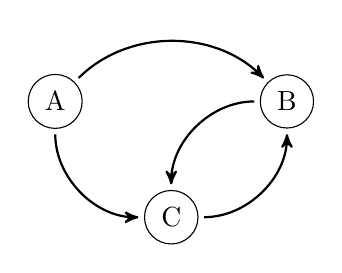
\begin{tikzpicture}[
roundnode/.style={circle, draw=black, thin},
]
%Nodes
\node[roundnode](C){C};
\node[above=of C](dummy){};

\node[roundnode](A)[left=of dummy]{A};

\node[roundnode](B)[right=of dummy]{B};

\path[pil] (A) edge [bend right=45] (C);
\path[pil] (B) edge [bend right=45] (C);
\path[pil] (C) edge [bend right=45] (B);
\path[pil] (A) edge [bend left=45] (B);

\end{tikzpicture}
\end{center}

\noindent Answer: Transition matrix
\begin{center}
\begin{tabular}{ |l|l|l|l| }
    \hline
      & A  & B  & C \\
    \hline
    A & 0  & 1  & 1  \\
    B & 0  & 0  & 1  \\
    C & 0  & 1  & 0  \\
    \hline
\end{tabular}
\end{center}

\noindent Transition probability matrix
\begin{center}
\begin{tabular}{ |l|l|l|l| }
    \hline
      & A    & B  & C \\
    \hline
    A & 0    & 0.5 & 0.5  \\
    B & 0    & 0   & 1    \\
    C & 0    & 1   & 0    \\
    \hline
\end{tabular}
\end{center}

\noindent Transition probability matrix with teleporting
\begin{center}
\begin{tabular}{ |l|l|l|l| }
    \hline
      & A    & B    & C      \\
    \hline
    A & 0.03  & 0.483 & 0.483  \\
    B & 0.03  & 0.03  & 0.933 \\
    C & 0.03  & 0.933 & 0.03  \\
    \hline
\end{tabular}
\end{center}

$$x = [1,0,0]$$
$$xP = [0.03, 0.48, 0.48]$$
$$xP^2 = [0.03, 0.48, 0.48]$$

\noindent \textbf{Question 4d} Compare language models with vector space models, both for information retrieval.

\noindent Not in syllabus\\

\noindent \textbf{Question 4e} Explain the crawling for Web search engines works, depicting communication between modules (or nodes) of crawling, including both URL frontier and DNS.

\noindent Solution not provided

\end{multicols*}
\end{document}
